\documentclass[10pt]{article}
\usepackage{fullpage}
\usepackage{amsfonts}
\usepackage{amsmath}
\usepackage{amsthm}
\usepackage{graphicx}
\usepackage{color}
\usepackage{amssymb}
\usepackage{empheq}
\usepackage{mathrsfs}
\usepackage{enumerate}
\usepackage{tikz}
\usepackage{pgflibraryarrows}
\usepackage{pgflibrarysnakes}
\usepackage{upgreek}
\usepackage{tipa}
\usepackage{multicol}
\usepackage{verbatim}
\usepackage{floatrow}
\usepackage{gensymb}
\usepackage{caption}

\usepackage{versions}
\excludeversion{sol}
\includeversion{sol}
\newenvironment{solution}{
\sol\\{\sc{Solution:}}}{
$\hfill\blacksquare$\endsol}

\newcommand{\de}[2]{\frac{d #1}{d #2}}

\usepackage[T1]{fontenc}
\usepackage[font=small,labelfont=bf,tableposition=top]{caption}

\DeclareCaptionLabelFormat{andtable}{#1~#2  \&  \tablename~\thetable}



\newfloatcommand{capbtabbox}{table}[][\FBwidth]

\usepackage{fancyhdr}
\setlength{\headheight}{15.2pt}
\pagestyle{fancy}
\setlength\headsep{30pt}
\lhead{Homework 3}
%\chead{\today}
\rhead{MATH 210}

\title{\textbf{\textsc{Homework 3}}\\
Differential Equations }
\author{\textbf{\textsc{MATH 210-010 $\diamond$ Fall 2024}}}
%\date{\today}



\begin{document}
\maketitle
\author

\vspace{3cm}
\begin{center}
\textsc{Due: Tuesday, October 22, 2024 }\\
%\textsc{Read: Matlab Week 1 Handout}
\end{center}


\normalsize
% \fbox{\fbox{\parbox{5.5in}{
 
        {\bf Instructions:}   To complete a problem set, you must submit a zip file labeled \verb|Yourlastname_HW#| to Dropbox no later than 11:59 PM on the due date above.  For example, if I were to complete this assignment, my folder would be named \verb!Emerick_HW3!.  In this folder, a \texttt{py} file is to be submitted for each problem such that when the \texttt{py} file is executed, the output (as presented in Python) is the solution to the problem.  Each \texttt{py} file must be saved as \verb!Yourlastname_HW#_No#.py!.  For example, if I were submitting the answer to Question Number 1 on Homework 3, the \texttt{py} file for that problem would be saved as \verb!Emerick_HW3_No1.py!.  Each \texttt{py} file should be well commented and be free of extraneous lines and commands.  Also, each \texttt{py} file must output only what the problem asked to be outputted.  Failure to abide by these simple homework submission guidelines may result in a deduction of points at my discretion.





%\vspace{4cm}
%\noindent \textsc{Instructions:}  To complete a problem set, you must submit a folder labeled \verb!Yourlastname_PS#! to Dropbox no later than midnight on the due date above.  For example, if I were to complete this assignment, my folder would be named \verb!Emerick_PS1!.  In this folder, an \texttt{m-file} is to be submitted for each problem such that when the \texttt{m-file} is executed, the output (as presented in \textsc{Matlab}) is the solution to the problem.  Each \texttt{m-file} must be saved as \verb!Yourlastname_PS#_No#.m!.  For example, if I were submitting the answer to Question Number 1 on Problem Set 1, the \texttt{m-file} for that problem would be saved as \verb!Emerick_PS1_No1.m!.  Each \texttt{m-file} should be well commented and be free of extraneous lines and commands.  Also, each \texttt{m-file} must output only what the problem asked to be outputted.  Failure to abide by these simple homework submission guidelines may result in a deduction of points at my discretion.  Remember:  if you don't know what a command does, you can always use \textsc{Matlab}'s \texttt{help} command or the internet...   \\

\vspace{2cm}
\flushright Name: $\qquad \qquad \qquad \qquad $
\flushright Score: $\qquad \qquad \qquad \qquad $

\pagebreak







\flushleft
%%%%%%%%%%%%%%%%%%%%%%%%%%%%%%%%%%%%%%%%%%
For each problem below submit a separate \texttt{py} file with an initial comment that describes the objective of the \texttt{py} file.  Always remember to begin your \texttt{py} file by importing appropriate libraries.  

\begin{enumerate}[{$\qquad 1.]$}]

\item Create a file that computes the numerical solution to the following initial value problem
\[ \de{y}{t} = ky\left(1-\frac{y}{M}\right)\left(\frac{y}{m} - 1\right)\, \qquad y(0) = y_0,\]
for parameter values $k>0$, $m>0$, and $M>0$ and an initial value $y_0$.  Your file should plot the solution to the equation with at least three solutions on the same graph, one with $y_0<m$, $m<y_0<M$, and one with $y_0>M$. 






 \item Consider the following system of that describes a predator-prey dynamic: 
\begin{align*}
\de{x}{t} & = Rx - 4x^2 - 3xy\\ 
\de{y}{t} & = -2y + xy \end{align*}
where $R>0$ is a real-valued parameter.  In this model, which population is the prey and which is the predator?  Plot the vector field with the phase plane solution as well. Briefly justify your answer.  Determine a value of $R$ that makes both populations coexist. 


\item The following schematic represents a chemical process in which a parent peptide (denoted by $P$) breaks down into four smaller components (denoted by $P_i$ for $i = 1, 2, 3, 4$).  The larger components can also break down into smaller components, where $P_4$ is the smallest component.  Here, assume each ``bin'' is a function of time and measures the concentration of each component in the solution.  
\begin{center}
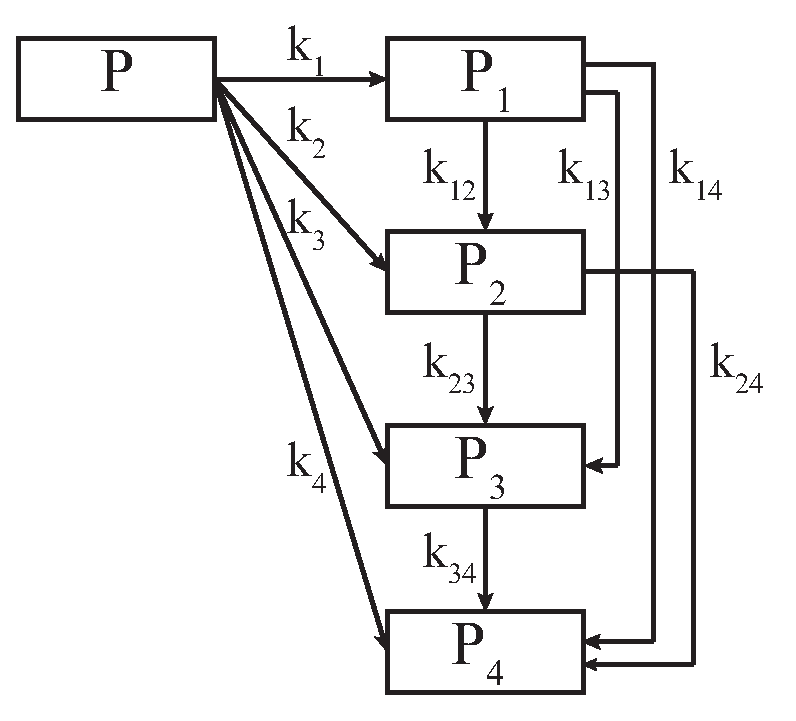
\includegraphics[width = .3\textwidth]{Peptide_Final_Schematic.eps}
\end{center}
Assume that the initial condition contains only the parent peptide, $P(0) = 1$, and all other components are not yet formed: $P_i(0)  = 0$ for $i = 1, 2, 3, 4$.  Set up and write down the linear differential equation model that simulates this process.  Assume each reaction is constant and positive.  Create a file that solves this model and outputs the solution when $k_1 = .09$, $k_2 = .8$, $k_3 = .07$, $k_4 = .6$, $k_{12} = .05$, $k_{13} = .5$, $k_{14} = .06$, $k_{23} = .7$, $k_{24} = .08$, and $k_{34} = .9$.  
\end{enumerate}










































\end{document}